\ifx \globalmark \undefined %% This is default.
\documentclass[a4paper,12pt]{report}

%%% PACKAGES %%%

\usepackage[french, english] {babel}	% langue principale
\usepackage[ansinew]{inputenc}
\usepackage[T1]{fontenc}		% Police contenant les caractères français
\usepackage{lmodern}			% plus beau
\usepackage[a4paper]{geometry}
	\geometry{hscale=0.75,vscale=0.8,centering}

\usepackage[hidelinks]{hyperref} % pas de couleurs ici
%
\usepackage[natbibapa]{apacite}

%% Maths
\usepackage{amsfonts} % Equations etc
\usepackage{amsmath}
\usepackage{mathtools}
\usepackage{amssymb}

\usepackage{cleveref}

%% Itemizes
\usepackage{enumerate}
\usepackage{enumitem}

%% Dessins & Plots
\usepackage[pdftex]{graphicx} %Images dans le PDF
\usepackage{epstopdf}
\usepackage{color, xcolor}
%% Dates
\usepackage{datetime}
\newdateformat{monthyeardate}{\monthname[\THEMONTH] \THEYEAR}
\usepackage{chessboard}
\usepackage{booktabs,tabularx,multirow}
\usepackage[babel=true,kerning=true]{microtype}
%> Tikz
\usepackage{tikz}
\usepackage{hf-tikz}
\usetikzlibrary{
	calc,
	arrows,
	arrows.meta,
	automata,
	shapes,
	snakes,
	positioning,
	decorations,
	decorations.text,
	fit,
	matrix,
	mindmap
	}
	\tikzstyle{noeud-std}=[draw,fill=black,circle,inner sep=0pt,minimum size=7pt]% 7pt est la taille des cercles noirs
\usepackage{tkz-graph}
\newcommand{\tikzmark}[2]{\tikz[overlay,remember picture,baseline=(#1.base)] \node (#1) {#2};}
\newcommand{\Highlight}[1][submatrix]{%
    \tikz[overlay,remember picture]{
    \node[highlight,fit=(left.north west) (right.south east)] (#1) {};}
    }
\tikzset{%
  highlight/.style={rectangle,rounded corners,fill=ocre!50,draw,
    fill opacity=0.5,thick,inner sep=0pt}
}
\newcommand{\mytikzmark}[2]{\tikz[overlay,remember picture, baseline=(#1.base)] \node (#1) {#2};}


%% Meta
\usepackage{etoolbox}

% Debugging purposes: Catch when a reference is missing
\makeatletter
	\patchcmd{\@setref}{\bfseries ??}{{\color{red}[\texttt{\detokenize{ #3 }}]}}{}{%
	  \GenericWarning{}{Failed to patch \protect\@setref}}
	\patchcmd{\@citex}{\bfseries ?}{{\color{red}[\texttt{\detokenize{ #3 }}]}}{}{%{{\color{red}\texttt{\@citeb}}}{}{%
	  \GenericWarning{}{Failed to patch \protect\@citex}}
\makeatother

%% CUSTOM ENVIRONMENTS
% Packages
\usepackage{framed}
\usepackage{mdframed}
\usepackage[amsmath,thref, framed]{ntheorem}

%% Counters for theorem.
% The current choice is that all environments share a counter within chapters.
% It that regards, it becomes easy to navigate the document.

\newcounter{theo}[chapter]\setcounter{theo}{0}
\renewcommand{\thetheo}{\arabic{chapter}.\arabic{theo}}



% The following is adapted from https://texblog.org/2015/09/30/fancy-boxes-for-theorem-lemma-and-proof-with-mdframed/
% \newenvironment{name}[args]{begin_def}{end_def}
\newenvironment{generic_theo}[2][] % 2 arguments, and one is optional. The first argument will say if we have a Thm or somth, the second is the name of the thm.
	{% begin_def
		\refstepcounter{theo}%
		\ifstrempty{#2} % looking at the name of the thm
		{
			\mdfsetup{
				frametitle={
					\tikz[baseline=(current bounding box.east),outer sep=0pt]
					\node[anchor=east,rectangle,fill=white!20, draw = black!20, line width = 2pt]
					{\strut #1~\thetheo};}
			} % The #1 will say Theorem, or other.
		}
		{
			\mdfsetup{
				frametitle={
				\tikz[baseline=(current bounding box.east),outer sep=0pt]
				\node[anchor=east,rectangle,fill=white!20, draw = black!20, line width = 2pt]
				{\strut #1~\thetheo:~#2};}
			}
		}
		\mdfsetup{innertopmargin=10pt,linecolor=black!20,
					linewidth=2pt,topline=true,
					frametitleaboveskip=\dimexpr-\ht\strutbox\relax
				}
\begin{mdframed}[]\relax}{\end{mdframed}}


%% Proofs (slightly different)
\newenvironment{generic_proof}[2][] % 2 arguments, and one is optional. The first argument will say if we have a Thm or somth, the second is the name of the thm.
	{% begin_def
		\refstepcounter{theo}%
		\ifstrempty{#2} % looking at the name of the thm
		{
			\mdfsetup{
				frametitle={
					\tikz[baseline=(current bounding box.east),outer sep=0pt]
					\node[anchor=east,rectangle,fill=black!20]
					{\strut #1~\thetheo};}} % The #1 will say Theorem, or other.
		}
		{
			\mdfsetup{
				frametitle={
				\tikz[baseline=(current bounding box.east),outer sep=0pt]
				\node[anchor=east,rectangle,fill=black!20]
				{\strut #1~\thetheo:~#2};}}
		}
		\mdfsetup{innertopmargin=10pt,linecolor=black!20,
					linewidth=1pt,topline=true,
					frametitleaboveskip=\dimexpr-\ht\strutbox\relax
				}
\begin{mdframed}[]
}{\end{mdframed}}

%% Examples/Exercices
\newenvironment{generic_ex}[2][] % 2 arguments, and one is optional. The first argument will say if we have a Thm or somth, the second is the name of the thm.
	{% begin_def
		\refstepcounter{theo}%
		\ifstrempty{#2} % looking at the name of the thm
		{
			\mdfsetup{
				frametitle={
					\tikz[baseline=(current bounding box.east),outer sep=0pt]
					\node[anchor=east,rectangle,fill=black!20]
					{\strut #1~\thetheo};}} % The #1 will say Theorem, or other.
		}
		{
			\mdfsetup{
				frametitle={
				\tikz[baseline=(current bounding box.east),outer sep=0pt]
				\node[anchor=east,rectangle,fill=black!20]
				{\strut #1~\thetheo:~#2};}}
		}
		\mdfsetup{innertopmargin=10pt,linecolor=black!20,
					linewidth=1pt,topline=true,
					frametitleaboveskip=\dimexpr-\ht\strutbox\relax
				}
\begin{mdframed}[]
}{\end{mdframed}}



% The different environments that we need (Main stuff are highlighted.
\newenvironment{theorem}[1][]{\begin{generic_theo}[Theorem]{#1}}{\end{generic_theo}}
\newenvironment{lemma}[1][]{\begin{generic_theo}[Lemma]{#1}}{\end{generic_theo}}
\newenvironment{definition}[1][]{\begin{generic_theo}[Definition]{#1}}{\end{generic_theo}}
\newenvironment{notation}[1][]{\begin{generic_theo}[Notation]{#1}}{\end{generic_theo}}
\newenvironment{proposition}[1][]{\begin{generic_theo}[Proposition]{#1}}{\end{generic_theo}}
\newenvironment{procedure}[1][]{\begin{generic_theo}[Procedure]{#1}}{\end{generic_theo}}
\newenvironment{hypothese}[1][]{\begin{generic_theo}[Hypothesis]{#1}}{\end{generic_theo}}


% These ones, let's not overblow them
% The true reason why I'm doing this is that there may be floats in Exercices and Examples...
% You can't have  begin{figures} in mdframed env, it crashes.
%\newtheorem{notation}[theo]{Notation}
\newcounter{axiomc}[chapter]\setcounter{axiomc}{0}
\renewcommand{\theaxiomc}{\arabic{chapter}.\arabic{axiomc}}

\newtheorem{axiom}[axiomc]{Axiom}
\newtheorem{proof}[theo]{Proof}
\newtheorem{exercise}[theo]{Exercise}
\newtheorem{example}[theo]{Example}



%% CUSTOM Commands

% Identify TAs
\newcommand{\TAone}{Mahsa}
\newcommand{\TAtwo}{Beno\^it}

\newcommand{\reels}{\mathbb{R}}

\DeclareMathOperator*{\argmin}{arg\,min}
\DeclareMathOperator*{\argmax}{arg\,max}

% Nice brackets
\newcommand\parent[1]{\left(#1\right)}
\newcommand\abs[1]{\left\lvert#1\right\rvert}
\newcommand\norm[1]{\left\lVert#1\right\rVert}
\newcommand\bracket[1]{\left\{#1\right\}}
\newcommand\squared[1]{\left[#1\right]}

\DeclarePairedDelimiter{\floor}{\lfloor}{\rfloor}
\DeclarePairedDelimiter{\ceil}{\lceil}{\rceil}
\usepackage{eurosym}
\usepackage{siunitx}
\DeclareSIUnit{\EUR}{\text{\euro}}
\sisetup{
  per-mode = fraction,
  inter-unit-product = \ensuremath{{}\cdot{}},
}



\usepackage{textcomp}
\let\texteuro\euro





\begin{document} %% Crashes if put after (one of the many mysteries of LaTeX?).
\else
\fi


\chapter{Evolutionary Game Theory}
\label{chap:Evol}
{\large{\itshape
``If you have an idea that was going to outrage society, would you keep it to yourself?''} --- Charles Darwin.\\
}
  {\small{\itshape
This chapter is inspired from \cite{NoED}.  Figures are taken from this book.}\\
}
\emph{}

\section{Introduction}
In the seventies, people like
William Hamilton and Robert Trivers proposed to apply ideas from mathematical ecology,
or more generally life sciences, to Game Theory.  This has led to an important subfield of Game Theory (and quite disconnected from the rest of it)
called Evolutionnary Game Theory. Other main actors of the developments in Evolutionary Game Theory are John Maynard Smith
 \cite{SmPrTLOA} (a geneticist and biologist from the UK) and Karl Sigmund (a mathematician from Vienna).

Evolutionary Game Theory analyses special types of games where \emph{a large number of identical agents} are playing.
The payoff of a player, here called \emph{fitness}, (which depends on the strategies of the agent, and of the other agents playing,
like in classical Game Theory) determines the \emph{reproduction rates} of agents.
One is interested in the different proportions of agents playing different strategies asymptotically.
 These proportions are to be interpreted as an Equilibrium, in the sense of Game Theory.
 Moreover, Evolutionary Game Theory does not assume any rationality of the agents, and these agents interact randomly, reproducing themselves (or disappearing) dependently of their types and the types of their fellow agents.

This idea is directly borrowed from classical concepts in Ecology. Let us see an example: on Figure \ref{frequency} are represented two species; one of which having the ability to move, while the other one is static.  When there are not many agents in the pool, the agent with the ability to move takes a great advantage of it, and its fitness is high.  However, when many agents are present, the agents are bound to be static, whatever their initial capacities are, and the mobile agent looses its comparative advantage.  It thus makes sense to model the fitness (the rate of reproduction) of the agents as depending on the relative `concentrations' of the different agents.

\begin{figure}[hbtp] \
\centering
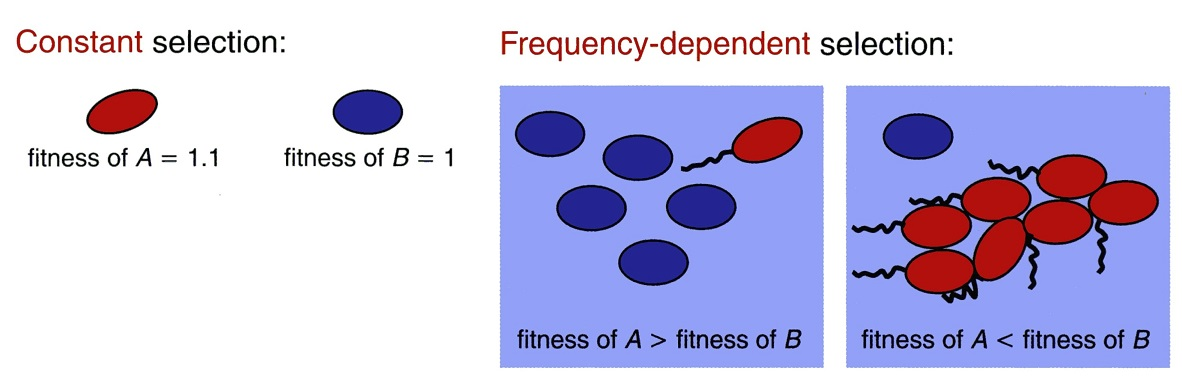
\includegraphics[scale=0.6]{im1.jpg}
\caption{Constant selection VS Frequency-dependent selection}
\label{frequency}
\end{figure}
Let us put formulas on this model, for two competing strategies $A$ and $B.$ Let  $x_A$ be the frequency of $A$ and $x_B$ be the frequency of $B.$The vector $\overrightarrow{x} = (x_A,x_B)$ defines the state of our dynamical system. In general, let the function $f_A(\overrightarrow{x})$ be the fitness of $A$ and $f_B(\overrightarrow{x})$ the fitness of $B.$ We note $\phi = x_A f_A(\overrightarrow{x})+ x_B f_B(\overrightarrow{x})$ be the average fitness. The laws of dynamics selection then write:
\begin{equation}
\begin{cases}
\dot{x}_A &= x_A \left[ f_A(\overrightarrow{x})-\phi \right] \\
\dot{x}_B &= x_B \left[ f_B(\overrightarrow{x})-\phi \right] \
\end{cases}
\label{syst}
\end{equation}

In what follows, we will only be interested in fitness functions depending on the \emph{relative} concentrations of each species.  Thus, we suppose that $x_A + x_B = 1$, and we can rewrite our dynamical system as a one-dimensional system with state-space variable $x$ such that : $x_A = x$ et $x_B = 1-x$. We have:
\begin{equation}
\dot{x} = x(1-x) \left[ f_A(x) - f_B(x) \right] \label{equa}
\end{equation}

The different equilibria of (\ref{equa}) are
\begin{itemize}
\item $x=0$, \item $x=1$ and \item all the values $x \in (0,1)$ such that $f_A(x) = f_B(x)$.\end{itemize} The equilibrium $x=0$ is stable if $f_A(0) < f_B(0)$ and the equilibrium $x=1$ is stable if $f_A(1) > f_B(1)$. Any other equilibrium $x^{\star}$ is stable if the functions $f_A$ et $f_B$ satisfy $f'_A(x^{\star}) < f'_B(x^{\star})$ (the functions are supposed to be twice differentiable). In general, there can be many equilibria in the interval $\left[ 0,1 \right].$ However, we will now restrict the shape of the functions $f_A(x),$ as they will be defined according to the game we are studying.
\section{Model and equilibria analysis}

How can we get inspiration from this biological example in order  to introduce a solution concept for two-player games?  We will consider our game from a new point of view: in evolutionary game theory, there is not a pair of players, playing one against each other, but rather, a large number of identical players, each of which having to pick a strategy in a common finite set.  This choice is their `DNA', and the impact of their choice is reflected in their ´reproduction rate', the probability that they will be able to reproduce themselve, given their DNA, and given the ecological system defined by the other players' choice.  Just like in classical game theory, the choice of other players will impact the `payoff' (here, the reproduction rate), of each player.  Hence, the payoff matrix can only be symmetric, since it does not represent several different players, but the payoff that each of them will receive, when facing one of their fellow agents. As a consequence, in Evolutionary Game Theory, one represents the payoff matrix in the following simplified way:
\begin{equation}
\begin{array}{l|cr}
 & A & B\\
\hline
A & a & b\\
B & c & d\\
\end{array}
\Longleftrightarrow
\begin{array}{l|cr}
 & A & B\\
\hline
A & a,a & b,c\\
B & c,b & d,d\\
\end{array}.
\label{payoff}
\end{equation}

The main idea of Evolutionary Game Theory is to consider the payoff as a fitness, in a dynamical system where agents reproduce proportionnally to their fitness.  Knowing $x_A$, the frequency of agent A, and $x_B$, the frequency of agent B, the expected fitness of respectively, agents of type A and agents of type B will be:

\begin{equation}
\begin{cases}
f_A = a x_A + bx_B \\
f_B = cx_A + dx_B
\end{cases}.
\label{syst2}
\end{equation}

These equations constitute a crucial point in our modeling procedure, where we interpret our payoff matrix as an \emph{infinite population} game.  Indeed, we made here the assumption that the expected fitness of an agent can be reinterpreted as being the fitness of all the agents in the population.  This is a classical assumption in modeling, also sometimes called `fluid model'.
If we insert these equations (\ref{syst2}) in our dynamical system  (\ref{equa}), we obtain :
\begin{equation}
\dot{x} = x(1-x) \left[ (a-b-c+d)x+b-d\right]. \label{equadiff}
\end{equation}

Thus, we are now facing a particular case of Equation (\ref{equa}), where the dynamics are described by four parameters $a,b,c,d.$
It turns out that in this case, only five situations are possible.
\begin{theorem}
In an evolutionary dynamics model derived from a two-player game as in Equation \eqref{equadiff}, one of the five following situations occur:
\begin{enumerate}
\item A dominates B if $a>c$ et $b>d,$ and the whole population will turn into A-individuals.
\item B dominates A if $a<c$ et $b<d,$ and the whole population will turn into B-individuals.
\item A et B are bistables if $a>c$ et $b<d:$ depending of the initial proportion of A and B-individuals, the whole population will turn into individuals of the same type. The treshold between these two antagonistic situations is an unstable equilibrium, given by $x^*=(d-b)/(a-d-b+c).$
\item A et B coexist at equilibrium.  This happens if $a<c$ et $b>d.$  In this case there is only one stable equilibrium, given by $x^*=(d-b)/(a-d-b+c).$
\item A et B are neutral if $a=c$ et $b=d.$ in this situation the population do not evolve in time, whatever the initial conditions are.
\end{enumerate}
\end{theorem}
\begin{proof}
Left for exercise.
\end{proof}

\section{Evolutionary Stable Strategy (ESS)}

This concept, Introduced by John Maynard Smith, aims at translating to Game Theory the concept of robustness from Systems and Control.  More precisely, we consider now a large population of A-agents, and we will say that strategy A is \emph{Evolutionary Stable} if it is robust against mutation of a small fraction of its population into B-individuals.
In this section,, we are only interested in characterizing pure strategies.
\subsection{Two-Player games}

We begin with a Two-Player game for simplicity:
\begin{definition}
Consider the game (\ref{payoff}).  A strategy $A$ is \emph{Evolutionnary Stable} (in short, ESS), if a population constituted initially of only $A$-individuals is stable under the mutation of an $\epsilon$ fraction of this population to another type of individual.
\end{definition}
Mathematically, let us consider a population composed of invading individuals B, so that   $x_B=\epsilon$, in an initial population of A-agents, so that $x_A=1 - \epsilon$. In this situation, the fitness of A is greater than the fitness of B if:
\begin{itemize}
\item \begin{equation}
\forall \epsilon>0, \, a(1-\epsilon) + b \epsilon > c(1-\epsilon)+d\epsilon \label{inegalite}
\end{equation}
and thus:
\begin{equation}
a > c
\end{equation}
\item or, if
$a=c$, we have
\begin{equation}
b>d.
\end{equation}
\end{itemize}
We can thus conclude:

\begin{proposition} A is an Evolutionary Stable Strategy if one of the following conditions is satisfied:
\begin{enumerate}
\item $a>c$
\item $a=c$ et $b>d.$
\end{enumerate}
\end{proposition}
\subsection{More than two strategies}
Let us generalize our analysis to games with more than two strategies.  In this case, the payoff for Strategy $S_i$ against Strategy $S_j$ is given by: $E(S_i,S_k)$ $\forall i \neq k$. We have:

\begin{enumerate}
\item Strategy $S_k$ is a strict nash equilibrium if:
\[E(S_k,S_k) > E(S_i, S_k)~~ \forall i \neq k\]
\item Strategy $S_k$ is a Nash equilibrium if :
\[E(S_k,S_k) \geq E(S_i,S_k) \ \forall i\]
\item Strategy $S_k$ is an ESS if $\forall i \neq k$ one has either :
\[E(S_k,S_k) > E(S_i, S_k)\]
or
\[E(S_k,S_k) = E(S_i,S_k)~\text{and}~ E(S_k,S_i) > E(S_i, S_i)\]
\item Strategy $S_k$ is stable against invasion (or `weak ESS') if $\forall i \neq k$ one has either:
\[E(S_k,S_k) > E(S_i,S_k)\]
or
\[E(S_k,S_k) = E(S_i,S_k)~\text{and}~E(S_k,S_i) \geq E(S_i,S_i)\] .\label{point}
\end{enumerate}
Point \ref{point} represents the case where A will not be eliminated by B, but, on the other hand, A won't manage to eliminate a small fraction of mutant B agents.  In this case both species will finally co-exist asymptotically.
%
%\subsection{Comparison with Nash Equilibria}
%We compare here the notion of Evolutionary Stable Strategy with the concept of Nash equilibria for the corresponding 2-Player Zero Sum game.  Recall that a \emph{strict Nash Equilibrium}  is a Nash Equilibrium where the inequalities in the definition are replaced with strict inequalities.
%Straightforward calculations give the following criteria for a game described as in (\ref{payoff}):
%\begin{enumerate}
%\item A is a strict Nash Equilibrium if $a>c$
%\item A is a Nash Equilibrium if $a \geq c$
%\item B is a strict Nash Equilibrium if $d>b$
%\item B is a Nash Equilibrium if $d \geq b.$
%\end{enumerate}

Summarizing, it is easy to see the following implications between our different pure-strategies equilibria:
\begin{equation}
\text{strict Nash}~~\Rightarrow~~~\text{ESS}~~\Rightarrow~~\text{weak ESS}~~\Rightarrow~~\text{Nash}.
\end{equation}

\section{Replicator Dynamics}
Just like in game theory, we would like to mathematically represent the fact that sometimes a `mix' of strategies is a good representation of the actual outcome of the game.  To this purpose, we are going to analyse the System (\ref{syst}) in the whole state space, and not only in situations where the complete population (except an $\epsilon$  proportion) is composed of a single agent. Generalizing to a $n$-Player game, the expected payoff of stragegy $i$ is given by $f_i = \sum\limits_{j=1}^{n}x_j a_{ij}.$  The average payoff among all the strategies is given by $\phi = \sum\limits_{i=1}^{n}x_i f_i.$ Then, we obtain the so-called \emph{Replicator equation} (See Figure \ref{imrepli}):
\begin{equation}
\dot{x}_i = x_i (f_i - \phi)~~~i=1,\dots ,n. \label{replicator}
\end{equation}
Equation (\ref{replicator}) is defined on the simplex $S_n$ (i.e. $\{x: \sum\limits_{i=1}^{n} x_i =1\}$).  It is easy to see that by design, the interior of the simplex is invariant: a trajectory can converge towards the boundary of the simplex (representing the fact that a population is dying), but it will never exactly hit the boundary.
\begin{figure}[hbtp]
\centering
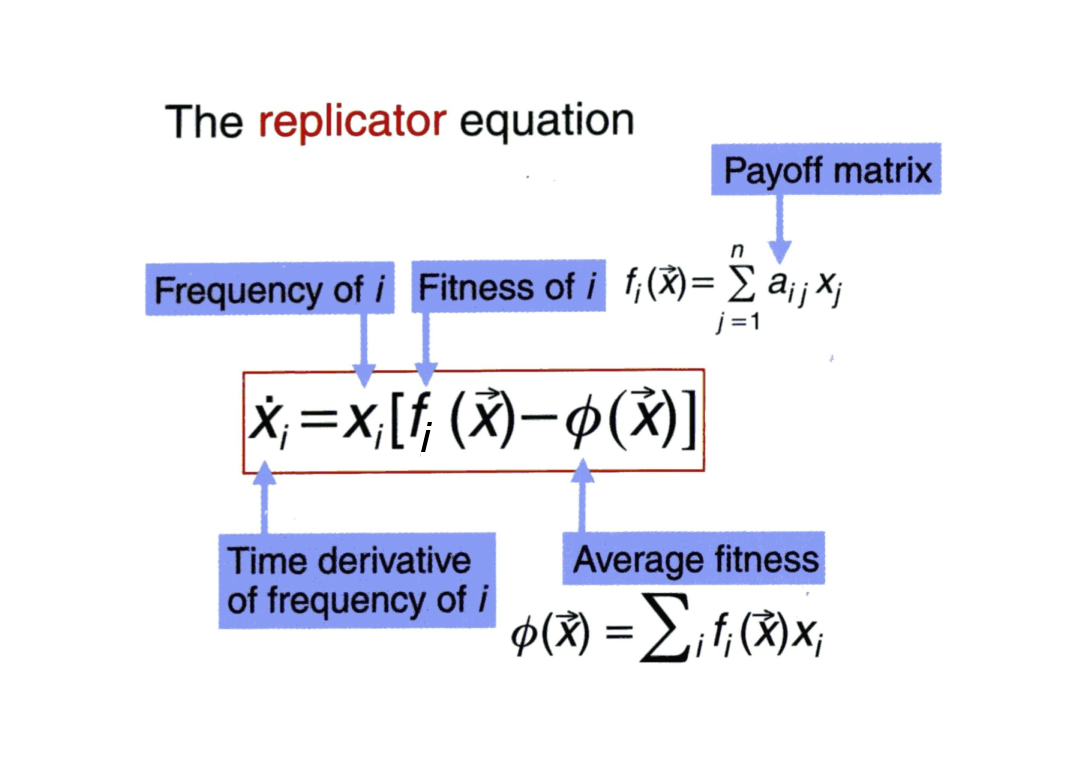
\includegraphics[scale=0.3]{im5.png}
\caption{The replicator equation}\label{imrepli}
\end{figure}
Let us now study how trajectories can behave.  For low dimensional systems, it is possible to completely characterize the behavior of all possible trajectories, depending on the values of the parameters.
\subsection{Two-strategies games}
%Le premier cas, lorsque $n=2$ a déjà été largement explicité dans ce résumé, mais reprenons-en l'essentiel. Considérons donc la matrice de payoff suivante
%\[
%\begin{pmatrix}
%	a_{11} & a_{12} \\
%	a_{21} & a_{22}
%\end{pmatrix}
%\]
The 2-Player case has been studied above: one can have fixed points in the interior of the simplex only if $(a_{11}-a_{21})(a_{12}-a_{22})<0.$ In that case, no population dominates the other one. This equilibrium is stable if $a_{11}<a_{12}$ and $a_{21}>a_{22}$. Obviously, in the neutral case ($a_{11}=a_{12}$ and $a_{21}=a_{22}$), all the points in the interval $[0,1]$ are equilibrium points.

\subsection{3-Player games}
If $n=3$, we have the following payoff matrix:
\[
\begin{pmatrix}
	0 & -a_{2} & b_{3} \\
	b_{1} & 0 & -a_{3} \\
	-a_{1} & b_2 & 0
\end{pmatrix}
\]
(Note that this matrix was obtained by subtracting from every column the corresponding diagonal element.  This will not change the equilibria, since the Replicator Equation \eqref{replicator} is also conserved.  One has thus the following possible cases:
\begin{itemize}
\item $a_1a_2a_3<b_1b_2b_3$
\item $a_1a_2a_3>b_1b_2b_3.$
\end{itemize}
In the first case, there exists a unique interior equilibrium which is globally stable.  In the second case, there exists a unique interior equilibrium which is unstable.
\subsection{Games with several strategies}
When $n>3$, one obtains the equilibria by solving these equations:
\[f_1 = f_2 = ... = f_n\]
\[x_1+x_2+...+x_n = 1.\]
This is a simple $n$-dimensional linear system.  Thus, there can at most be one single isolated equilibrium.
\subsection{Lotka-Volterra Equations}

Predator-Prey models have been developed by Vito Volterra, an italian physicist, just after WW2.  His goal was to understand a sudden rise in the concentration of sharks in the Adriatic sea following the war.  His equations represented populations of preys $x,$ and predators, $y.$  The preys reproduce at rate $a$ and are eaten at a rate $b,$ predators dying at a rate $c$ and reproducing at rate $d.$
\[\dot{x} = x(a-by)\]
\[\dot{y} = y(-c+dx)\]
First, if there are no predators, or no prey, the other populations evolve according to increasing (resp. decreasing) curves.

\[x(t)=x(0)e^{at}\]
\[y(t)=y(0)e^{-ct}\]
In the general case, we have the following interior stable equilibrium.
\[x^*=c/d\]
\[y^*=a/b\]
Now, if fishing decreases, the concentration of preys increases, which indirectly causes a rise in concentration of sharks.


Generalizing these equations to more than two species, one obtains the famous \emph{Lotka-Volterra equations:}
\[\dot{y_i}=y_i(r_i + \sum_{j=1}^n b_{ij}y_j).\]
It is easy to show that these equations are actually perfectly equivalent to the {\it{replicator equation}} \eqref{replicator}: Evolutionnary Game Theory is nothing more than Mathematical Ecology applied to Game Theory.
\subsection{An example: Hawk or Dove}
This paradigmatic game in Game Theory comes from Ecology: scientists wanted to understand and explain violence and domination in nature.  Violence can indeed be beneficial for an individual, if it allows him to enhance reproduction of its own genes, compared with other species.  Of course, it can also be harmful when two such individuals meet. We thus consider two species: hawks, and doves.  Each species can chose (through long term mutations) to fight everytime they meet another bird, of to flee. In the following payoff matrix, $b$ represents the payoff in case of victory, and $c$ represents the cost of injuries after loosing a fight.  Thus, the expected payoff when two hawks meet is $(b-c)/2.$  If a hawk meets a dove, the hawk wins, and thus receives a payoff of $b,$ while the dove doesn't engage, and hence leaves with a zero payoff. We thus have the following payoff matrix:
\[
\begin{pmatrix}
	\frac{b-c}{2} & b \\
	0 & \frac{b}{2}
\end{pmatrix}
\]
If $c>b$, there is no pure-strategy Nash equilibrium.  If every individual choses to play Hawk, playing dove is the best strategy, and vice versa.  Hence, there is a mixed population equilibrium, with a rate of hawks-individuals equal to $b/c.$
%
%\subsection{Chicken}
%Let us now consider another well-known game: the Chicken game.  We have already studied this game, which exhibits a 'prisonner's dilemma' phenomenon.  The payoff matrix is the following one:
%\[
%\begin{pmatrix}
%	-c & b \\
%	0 & \frac{b}{2}
%\end{pmatrix} \ \ \ \ \ \ \ \ \ \ \ \
%\begin{pmatrix}
%	b-\frac{c}{2} & b-c \\
%	b & 0
%\end{pmatrix}
%\]


\section{Finite population}
It is possible to rewrite all the conditions above, by supposing that the (large number of) identical agents is finite, instead of infinite.  Mathematically, one must then model the birth-death process in a stochastic way (as in so-called \emph{Moran} processes). By making use of similar notions of robustness to mutation-perturbations, one can define new notions of equilibria for a given (symmetric) payoff table.
Interestingly, this finite population assumption can lead to significantly different numerical values of equilibria.


\ifx \globalmark \undefined %% This is default.
\bibliographystyle{plain}
\bibliography{../gametheorybibliography}
\end{document}
\else

\fi
